\bluepage{WebGL}

\begin{frame}
\frametitle{WebGL}
	\begin{itemize}
	\item{OpenGL aplikace v prohlížeči}
	\item{API pro 3D grafiku v prohlížeči}
	\item{Programuje se v Javascriptu}
	\item{OpenGL ES}
	\end{itemize}
\end{frame}

\begin{frame}
\frametitle{WebGL - Voda}
	\begin{figure}[h]
	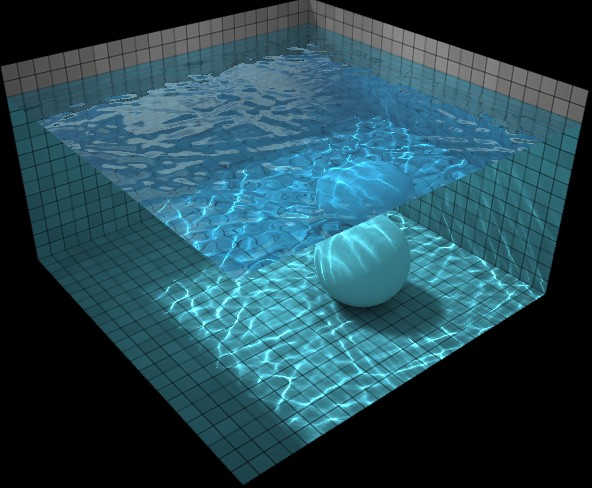
\includegraphics[width=10cm,keepaspectratio]{pics/webgl_water.jpg}
	\end{figure}
\end{frame}

\begin{frame}
\frametitle{WebGL - Modely z doom 3}
	\begin{figure}[h]
	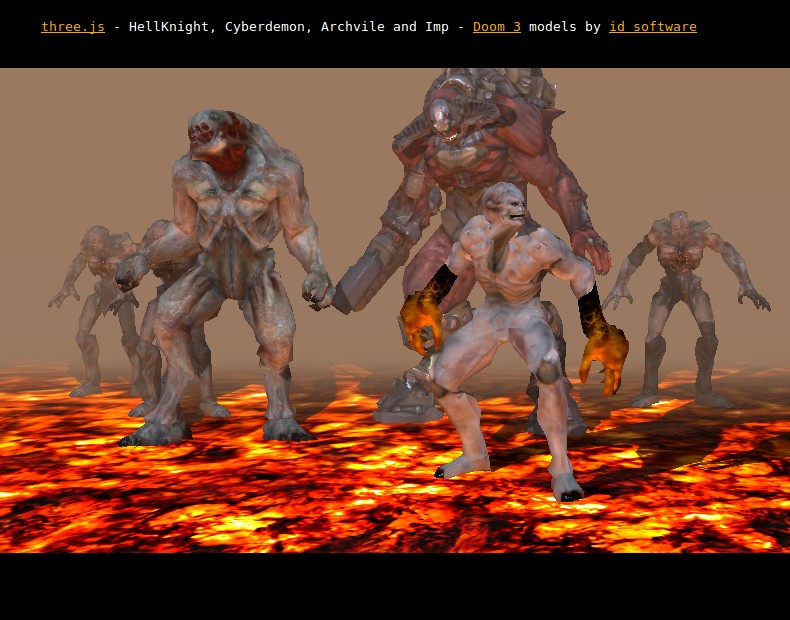
\includegraphics[width=10cm,keepaspectratio]{pics/webgl_doom.jpg}
	\end{figure}
\end{frame}


\begin{frame}
\frametitle{WebGL - OpenGL v Prohlížeči}
	\begin{itemize}
	\item \url{http://www.chromeexperiments.com/webgl/}
	\item \url{http://madebyevan.com/}
	\item \url{https://www.shadertoy.com/}
	\item \url{http://playwebgl.com/}
	\item \url{http://media.tojicode.com/q3bsp/}
	\item \url{http://alteredqualia.com/three/examples/webgl_animation_skinning_doom3.html}
	\item \url{...}
	\end{itemize}
\end{frame}

\begin{frame}[fragile]
\frametitle{WebGL - příklad}
		Soubor webgl.js
		{\scriptsize
		\begin{minted}[frame=lines]{javascript}
		var gl;//objekt gl
		var program;//shader program
		var VBO;//vertex buffer object

		//funkce pro inicializaci WebGL
		function initGL(canvas){
		  try{
		    gl=canvas.getContext("experimental-webgl");//kontext
		    gl.viewportWidth=canvas.width;//sirka view portu
		    gl.viewportHeight=canvas.height;//vyska view portu
		  }catch(e){
		  }
		  if(!gl){
		    alert("Could not init WebGL");
		  }
		}
		\end{minted}
		}
\end{frame}

\begin{frame}[fragile]
\frametitle{WebGL - příklad pokračování}
		Soubor webgl.js
		{\scriptsize
		\begin{minted}[frame=lines]{javascript}
		//funkce vytvori shader program
		function CreateShaderProgramVSFS(vertexSource,fragmentSource){
		  var vshader=gl.createShader(gl.VERTEX_SHADER);//vertex shader
		  var fshader=gl.createShader(gl.FRAGMENT_SHADER);//fragment shader
		  gl.shaderSource(vshader,vertexSource);//nahrani zdrojaku v. shaderu
		  gl.shaderSource(fshader,fragmentSource);//nahrani zdrojaku f. shaderu
		  gl.compileShader(vshader);//kompilace vertex shaderu
		  gl.compileShader(fshader);//kompilace fragment shaderu
		  if(!gl.getShaderParameter(vshader,gl.COMPILE_STATUS))
		    alert(gl.getShaderInfoLog(vshader));//chyba
		  if(!gl.getShaderParameter(fshader,gl.COMPILE_STATUS))
		    alert(gl.getShaderInfoLog(fshader));//chyba

		  var programID=gl.createProgram();//vytvorime novy shader program
		  gl.attachShader(programID,vshader);//pripojime vertex shader
		  gl.attachShader(programID,fshader);//pripojime fragment shader
		  gl.linkProgram(programID);//slinkujeme shader dohromady
		  if(!gl.getProgramParameter(programID,gl.LINK_STATUS))
		    alert("LINK ERROR");//chyba

		  return programID;//navrat shader programu
		}
		\end{minted}
		}
\end{frame}

\begin{frame}[fragile]
\frametitle{WebGL - příklad pokračování}
		Soubor webgl.js
		{\scriptsize
		\begin{minted}[frame=lines]{javascript}
		function WebGLStart(){
		  var canvas=document.getElementById("test");//ziskani platna
		  initGL(canvas);//inicializace WebGL
		  program=CreateShaderProgramVSFS(//vytvoreni programu
		      "attribute vec2 Pos;void main(){gl_Position=vec4(Pos,0,1);}",
		      "void main(){gl_FragColor=vec4(1,0,0,0);}");
		  gl.useProgram(program);//pouzijeme shader program
		  program.posatt=gl.getAttribLocation(program,"Pos");//atribut pozice
		  gl.enableVertexAttribArray(program.posatt);//povolime atribut pozice
		  VBO=gl.createBuffer();//vytvorime VBO
		  gl.bindBuffer(gl.ARRAY_BUFFER,VBO);//navazeme vytvorime VBO
		  var Data=[0,0,.3,.3,-.3,-.3,.3,-.3,-.3,.3];//data
		  gl.bufferData(gl.ARRAY_BUFFER,new Float32Array(Data),gl.STATIC_DRAW);
		  gl.clearColor(0,0,0,1);//cerna barva pozadi
		  gl.enable(gl.DEPTH_TEST);//depth test
		  gl.viewport(0,0,gl.viewportWidth,gl.viewportHeight);//nastaveni viewportu
		  gl.clear(gl.COLOR_BUFFER_BIT|gl.DEPTH_BUFFER_BIT);//vycistime framebuffer
		  gl.vertexAttribPointer(program.posatt,2,gl.FLOAT,false,0,0);//attibut
		  gl.drawArrays(gl.POINTS,0,5);//vykreslime 5 bodu
		}
		\end{minted}
		}
\end{frame}

\begin{frame}[fragile]
\frametitle{WebGL - příklad pokračování}
		Soubor index.html
		{\scriptsize
		\begin{minted}[frame=lines]{html}
		<!-- Soubor s WebGL !-->
		<script type="text/javascript" src="webgl.js">
		</script>

		<html>
		  <body onload="WebGLStart();">
		    <canvas id="test" style="border: none;" width="500" height="500"/>
		  </body>
		</html>

		\end{minted}
		}
\end{frame}

